Celý proces získání konkrétní entity pro potřeby aplikační vrstvy je postaven na~několika návrhových vzorech. Správné užití návrhových vzorů umožní zapouzdřit chování jednotlivých tříd, nebudou vytvářena těsná propojení jednotlivých tříd a celý zdrojový kód bude flexibilnější. Cílem tohoto přístupu je zjednodušení případných budoucích úprav aplikace. Těsné provázání tříd aplikační a databázové vrstvy sice znamená méně náročnou práci při první implementaci, ale o to je náročnější kód v~budoucnosti upravit. 

Příkladem může být objekt -- entita, který se umí perzistovat, tj. je přímo závislý na~konkrétní implementaci úložiště. Při změně úložiště je pak potřeba upravit všechny takové objekty.

\n{2}{Modelová vrstva}
Z pohledu architektury MVC reprezentuje modelová vrstva data a manipulaci s nimi a v aplikaci se výrazně překrývá s doménovou vrstvou z pohledu DDD. Způsob implementace byl zvolen tak, aby zbytek aplikace nebyl pevně spojen se způsobem získávání a ukládání dat (entit).

Single Responsibility Principle (Princip jedné odpovědnosti) zavedený Robertem~C.~Martinem udává, že ``třída by měla mít pouze jeden důvod ke změně''\footnote{A class should have only one reason to change\cite{Martin2002}}. Změnou je zde myšleno přepracování kódu. Pokud má třída pouze jednu odpovědnost, pouze ta může vyvolat nutnost změny kódu. Entita má odpovědnost podávat o sobě informace, její odpovědností není, jak je vytvořena, jak a jestli vůbec je perzistována v databázi či jinde atd. Vytváření entit by měla mít na starosti třída typu \phpinline{Factory}, převedení dat z~úložiště do formátu, kterému továrna rozumí je úkolem pro \phpinline{Data Mapper}. Získání entit pro potřeby aplikace je práce pro \phpinline{Repository}. 

Získávání a manipulace s entitami byla implementována pomocí návrhových vzorů Data Mapper a Repository. Aplikační vrstva (především Presentery) získává jako závislost repozitáře (třídy typu Repository), které jí poskytují požadované entity nebo kolekce entit. V souladu se SRP Presenter nezajímá, jakým způsobem jsou entity získávány, k jeho odpovědnosti to nepatří. Repozitáře vědí, že rozhraní Data mapper umí poskytovat entity bez ohledu na to, kde a jak je konkrétní entita uložena (v paměti, souboru, databázi či jinde). V aplikaci je pouze jedna implementace a to \phpinline{DbDataMapper}. Data mapper pomocí databázového adaptéru Dibi odesílá požadavky na databázový server. Vytváření entit je řešeno částečně továrními metodami data mapperů a částečně samotnými továrními třídami v závislosti na složitosti operace. Ideální by ovšem bylo striktní oddělení do samostatných tříd.

\begin{figure}[h]
	\centering
	\includegraphics[width=\linewidth]{svg/roleMapper.png}
	\captionsetup{width=\linewidth}
	\caption[Diagram modelové vrstvy]{Diagram modelové vrstvy (zdroj: vlastní)}
	\label{fig:RoleMapper}
\end{figure}

Diagram na obrázku \ref{fig:RoleMapper} obecně popisuje použité řešení, které bylo aplikováno na všechny entity. Třída \phpinline{RoleDbMapper} implementuje rozhraní \phpinline{RoleMapper}, které je předáno třídě \phpinline{RoleRepository} jako závislost. V diagramu je použit příklad role, vyhledat ji lze podle id nebo podle vazby na entitu \phpinline{User}. Vhodné například, pokud chceme zjistit, které konkrétní role má uživatel nastaveny a tedy k jakým prostředkům a akcím má přístup díky pravidlům přiřazeným k jeho daným rolím. Zde je vhodné připomenout diagram na obrázku \ref{fig:AclModel}, který popisuje vazby mezi uživatelem, rolemi atd.

Metody \phpinline{find(), findOne(), findAll()} a \phpinline{findRelated()} slouží k vyhledání entit podle zadaných parametrů. Těmi může být filtr na Id nebo společnou vlastnost ale i vazba na jinou entitu. Metoda \phpinline{getDataSource()} slouží k získání dat pro zobrazení interaktivních tabulek v administraci aplikace. Pomocí metody \phpinline{create()} dokáže vytvořit nové instance entity \phpinline{Role}, které jsou následně předány repozitáři samostatně (\phpinline{findOne()}) nebo jako kolekce (některé mappery předávají objekt \phpinline{...Collection}, některé předávají pole objektů).
\clearpage

\n{2}{Struktura databáze}
Pomocí stanovených modelů bylo možné navrhnout podrobnější modely jednotlivých entit a tím pádem i strukturu databáze.

\begin{figure}[h]
	\centering
	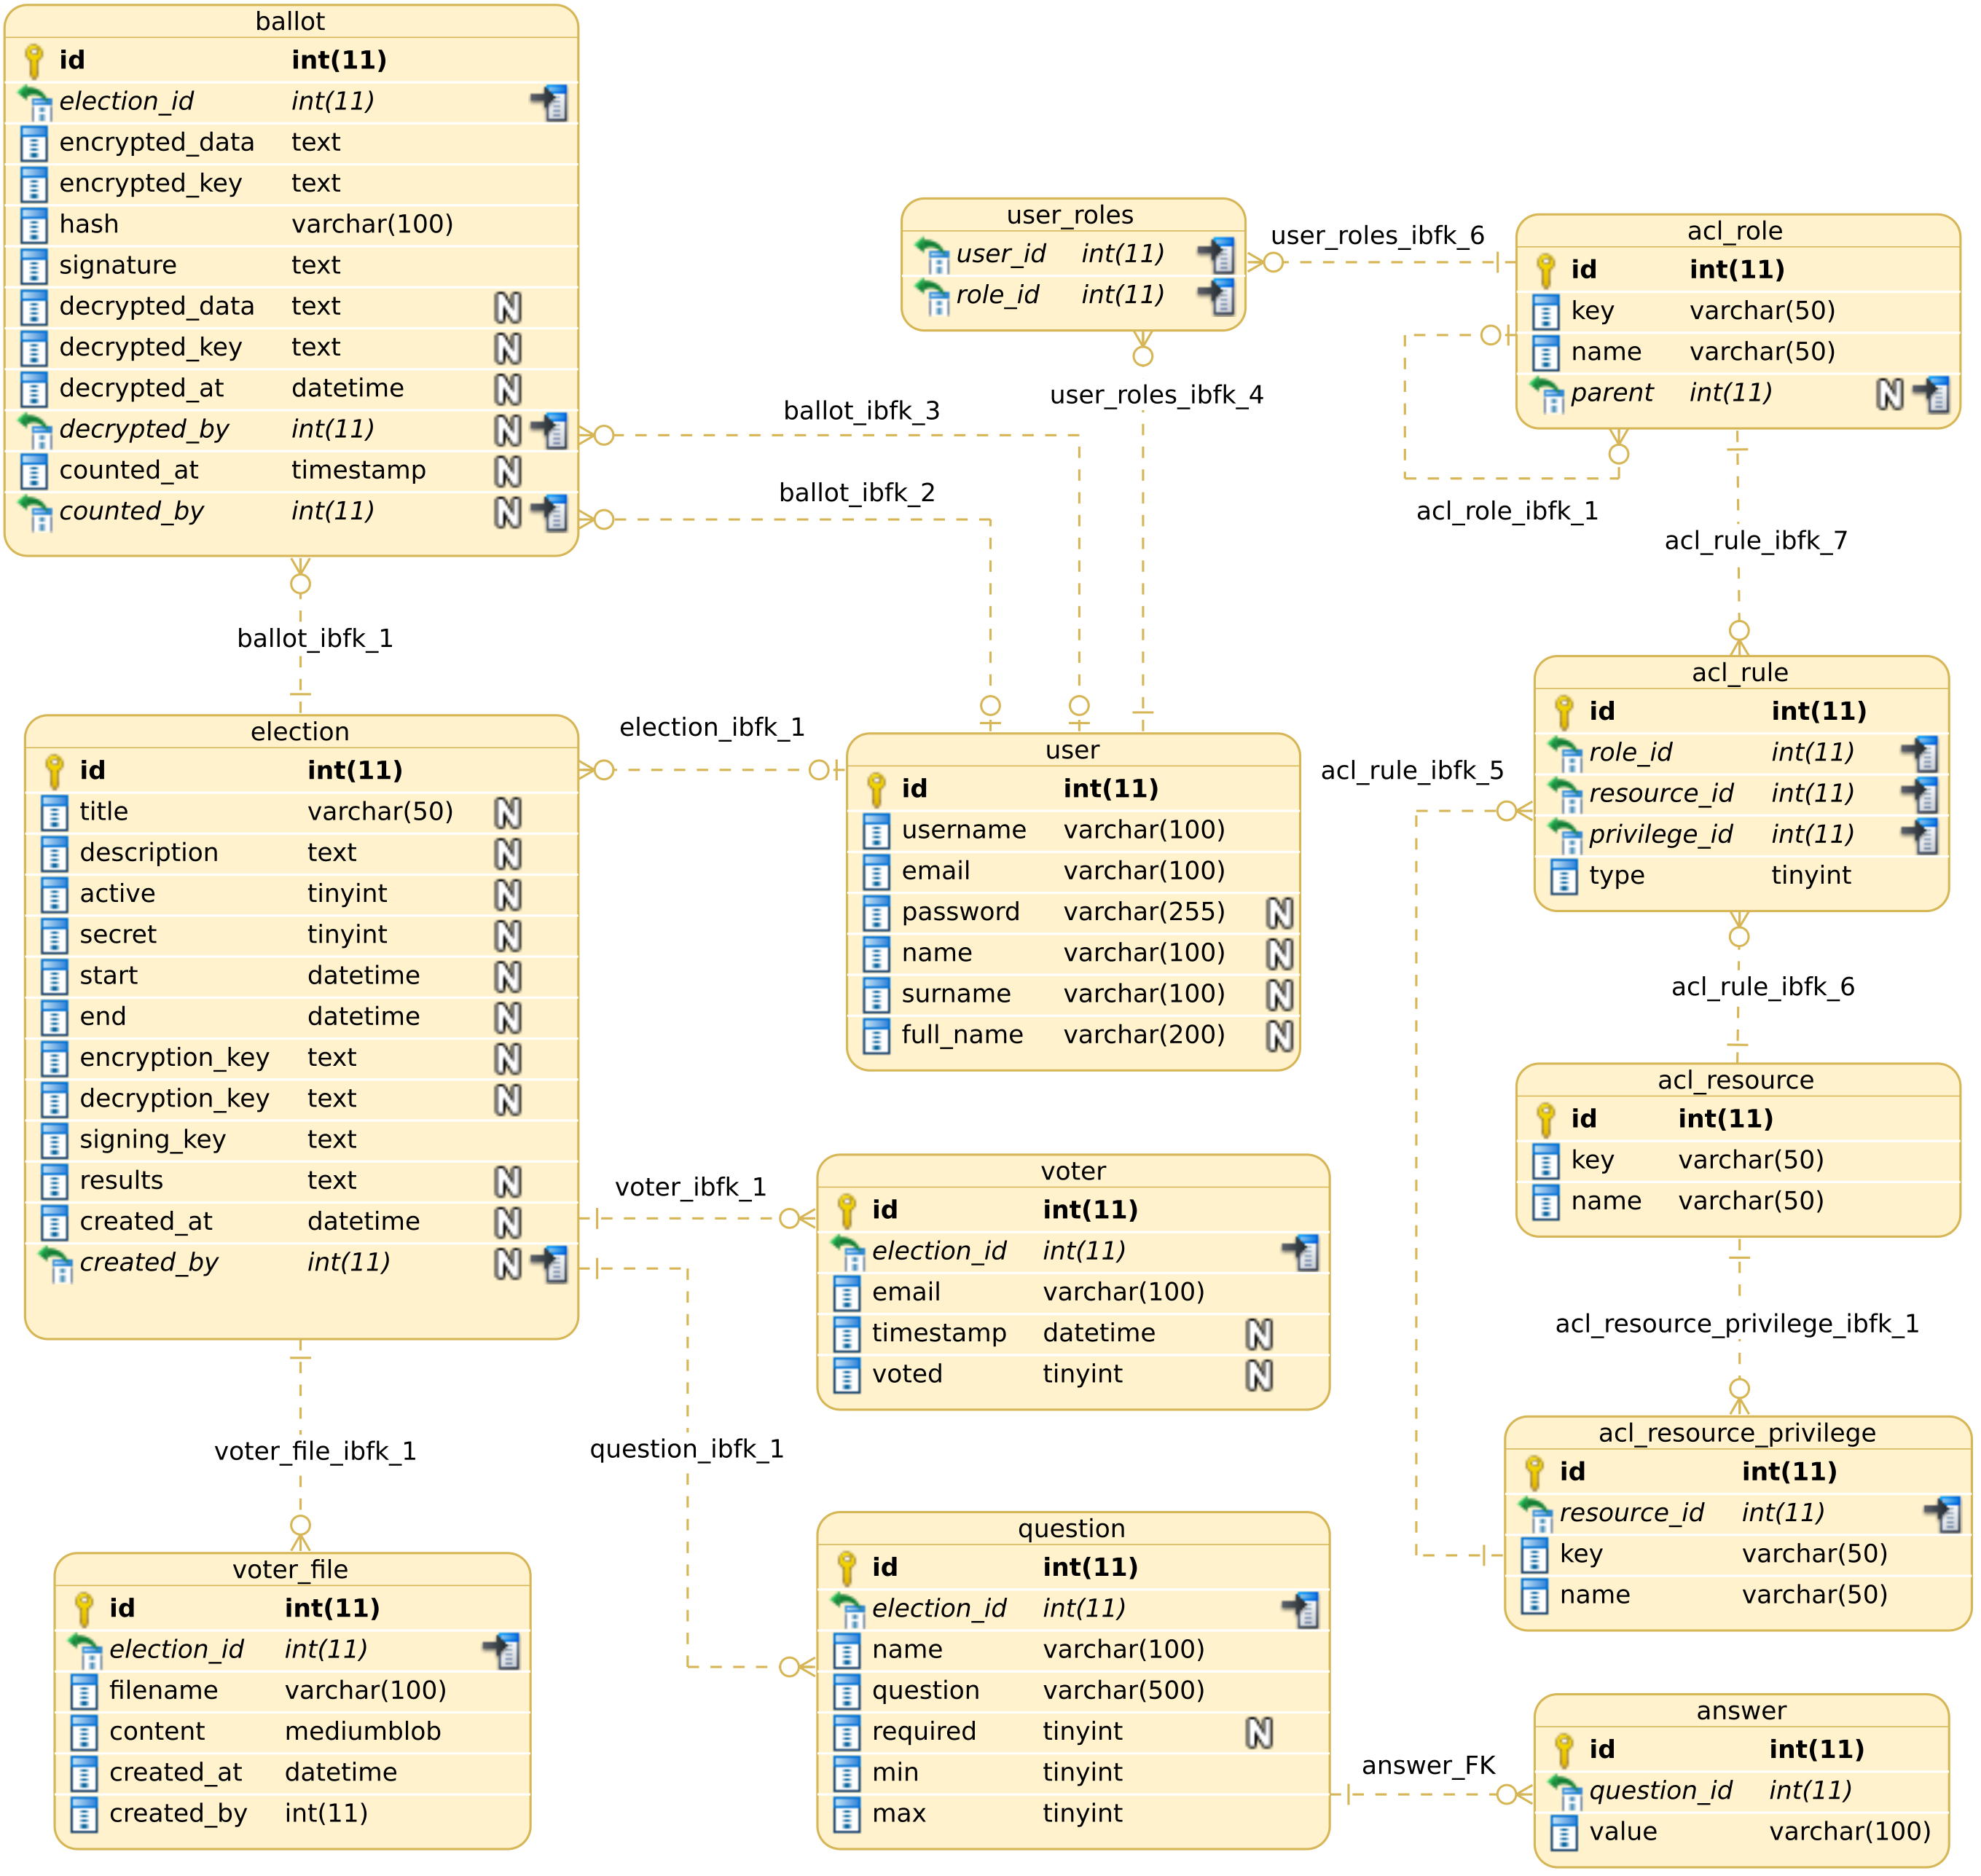
\includegraphics[width=\linewidth]{svg/erd3.png}
	\captionsetup{width=\linewidth}
	\caption[Entitně relační diagram]{Entitně relační diagram (zdroj: vlastní)}
	\label{fig:ERD}
\end{figure}


\clearpage